\documentclass[12pt,a4paper]{article}
\usepackage[utf8x]{inputenc}
\usepackage{ucs}
\usepackage{amsmath}
\usepackage{amsfonts}
\usepackage{amssymb}
\usepackage{graphicx}
\usepackage{listings}
\usepackage[left=2cm,right=2cm,top=2cm,bottom=2cm]{geometry}

\usepackage{natbib}
\bibpunct{[}{]}{,}{n}{}{;}

\usepackage[pdftex,pagebackref]{hyperref}
    \usepackage{natbib}
    \hypersetup{colorlinks,linktocpage=true}
\renewcommand{\backrefpagesname}{ \protect\\  \textit{Cited on
page(s):}~}
\renewcommand{\backref}{\backrefpagesname}

\author{Gergely Imreh}
\title{LabWeather}
\date{2013-03-21, v1}
\begin{document}
\maketitle

The purpose of the laboratory weather monitoring circuit was to double-check the air-conditioning system, and provide a quick overview to the (in)stability of the lab humidity and temperature.

\tableofcontents

\section{Sensors}

\subsection{Humidity sensor}

The humidity sensor used is a general CM-R resistive humidity sensor \footnote{CM-R spec sheet: \url{http://file.yizimg.com/3381/20061221103057890280486.pdf}}. Because of its design, it is not allowed to have any DC voltage across it. This could be achieved by driving it with AC voltage, or more reliably by decoupling with capacitors from the DC parts of the circuit

The current circuit is shown on Fig. \ref{fig:circuit}, part 1.

\begin{figure}[ht!]
\centering
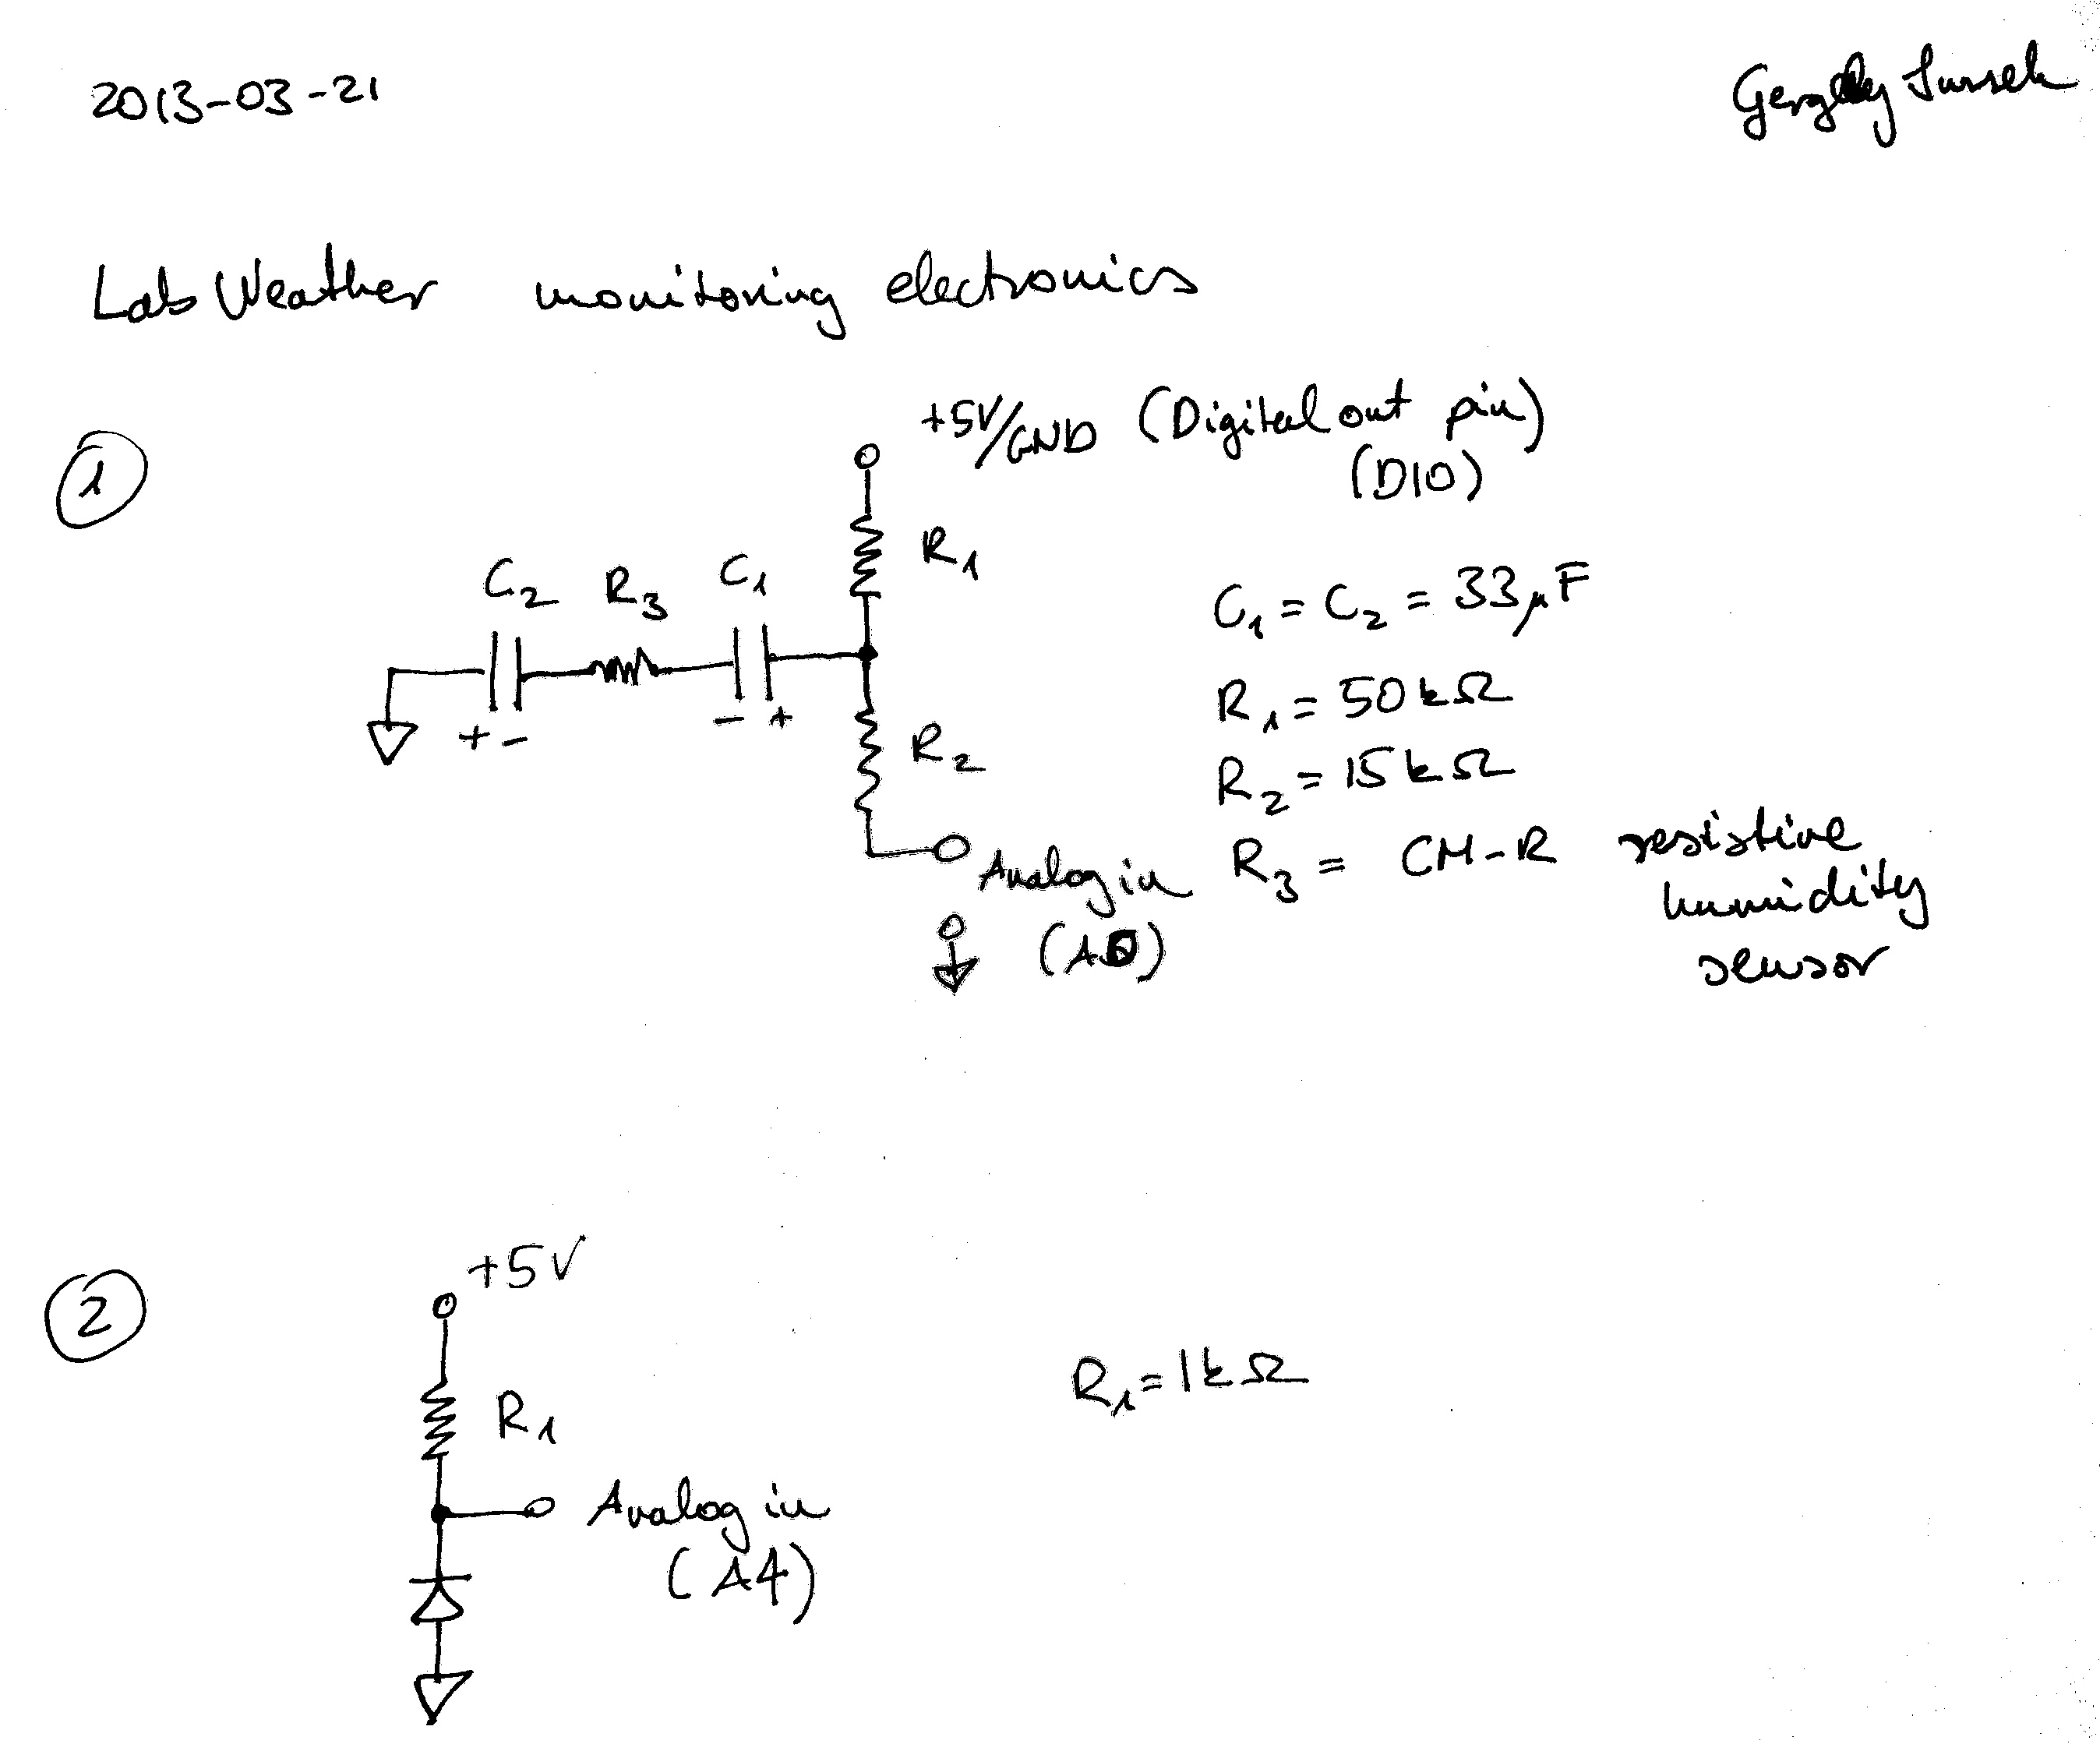
\includegraphics[width=140mm]{circuit.jpg}
\caption{The circuits for the lab weather monitoring setup}
\label{fig:circuit}
\end{figure}

To measure the resistance of the sensor, the controller is driving it at 1kHz with square waves, and at fixed intervals (current setting: every 1 second) the square wave is stopped and a quick resistance measurement is made, then the square wave is resumed. Since the sensor is working continuously for months without apparent change in behaviour, this seems to be safe enough.

The resistance value is from an analog voltage measurement in voltage divider arrangement with the known value of $R_1$, though it is complicated by the presence of decoupling capacitors. The voltage divider equation in this case is given by
\begin{equation}
V_{\rm in} - V_C = \left(V_{\rm cc} - V_C \right) \frac{R_3}{R_3 + R_1}
\end{equation}
where $V_{\rm in}$ is the measured voltage, $V_C$ is the voltage the capacitor is charged up by the AC input signal, $V_{\rm cc}$ is the supply voltage. In the current setting, $V_{\rm cc} = 5V$, $V_C = V_{\rm cc} / 2 = 2.5V$. Rearranging this equation for $R_3$:
\begin{equation}
R_3 = \frac{R_1}{\frac{V_{\rm cc} - V_C}{V_{\rm in} - V_C} - 1}
\end{equation}
From experience, $V_C$ is actually quite dependent on the measurement frequency, probably during the measurement the capacitors are discharging somewhat, which will lead to erroreous resistance value. With 2Hz measurement rate the measured resistance is $\approx 80\%$ of the true value, with 1Hz it is $\approx 90\%$, with 0.25Hz $\approx 97\%$. Since the humidity-vs-resistance curve is very steep, these differences have very small effect on the final outcome (likely below the accuracy of the sensor itself), to be more consistent, though, currently a correction factor of $1/0.9$ is applied (for the 1Hz measurement).

The recorded humidity values are consisted with other independent humidity measurements (HOBO U10\footnote{HOBO U10 product page: \url{http://www.onsetcomp.com/products/data-loggers/u10-003}}).

The humidity vs. resistance can be derived from the spec sheet, for recording purposes the current version is assuming $25\mathrm{^\circ C}$ temperature, which is close enough, $\approx \pm 5 \% $ error for our lab temperature range. Thus here it is
\begin{equation}
\mathrm{RH\%} =  2.76366367 \times (\log_{10} R) ^ 2 - 32.40924966 \times (\log_{10}R) + 102.93566686
\end{equation}
where the coefficients I got from fitting the spec sheet data.

Further improvement would be to rewire the sensor in an AC balanced bridge arrangement, but haven't had a chance to figure that one out.

\subsection{Temperature sensor}

Texas Instruments LM335\footnote{LM335 product page: \url{http://www.ti.com/product/lm335}} in the simplest possible arrangement. It can be considered as a regular Zener-diode, with temperature dependent breakdown voltage, in this case $10\mathrm{mV}/\mathrm{K}$. Thus room temperature gives about $2.93\mathrm{V}$ across it.

The circuit is shown on Fig. \ref{fig:circuit}, part 2.

One problem is that the currently used Arduino's ADC has only 10bits over 0-5V, only being able to resolve about $0.5\mathrm{^\circ C}$, with quite a bit of noise. Thus the measured value needs to be averaged and filtered for practical use.

Further improvement is possibe to amplify the signal around the usual working voltage. Most likely it would be an op-amp in single-supply mode. Tried one such circuit with 10x amplification, the temperature resolution is better, but the measurement noise (measured by calculating the standard deviation) is only reduced by half. Thus this might not worth the extra effort.

\section{Data relay}

The resistance and voltage measurements for the humidity and currently done with an Arduino Diecimilla\footnote{Arduino Diecimilla product page: \url{http://arduino.cc/en/Main/ArduinoBoardDiecimila}}. It is obsolete product now, but any other Arduino should do the trick, and even could build a barebones kit with the Atmel328 microcontroller chips with not too much effort.

The current source code can be found on the net\footnote{Humidity sensor source code: \url{https://github.com/UltracoldAtomsLab/weatherstation/tree/master/humidity1}}. When in doubt how to load that data onto the Arduino, consult it's Getting Started Guide\footnote{Arduino Getting Started: \url{http://arduino.cc/en/Guide/HomePage}}.

The Arduino sends the measured data to the computer via the attached USB cable.

\begin{figure}[ht!]
\centering
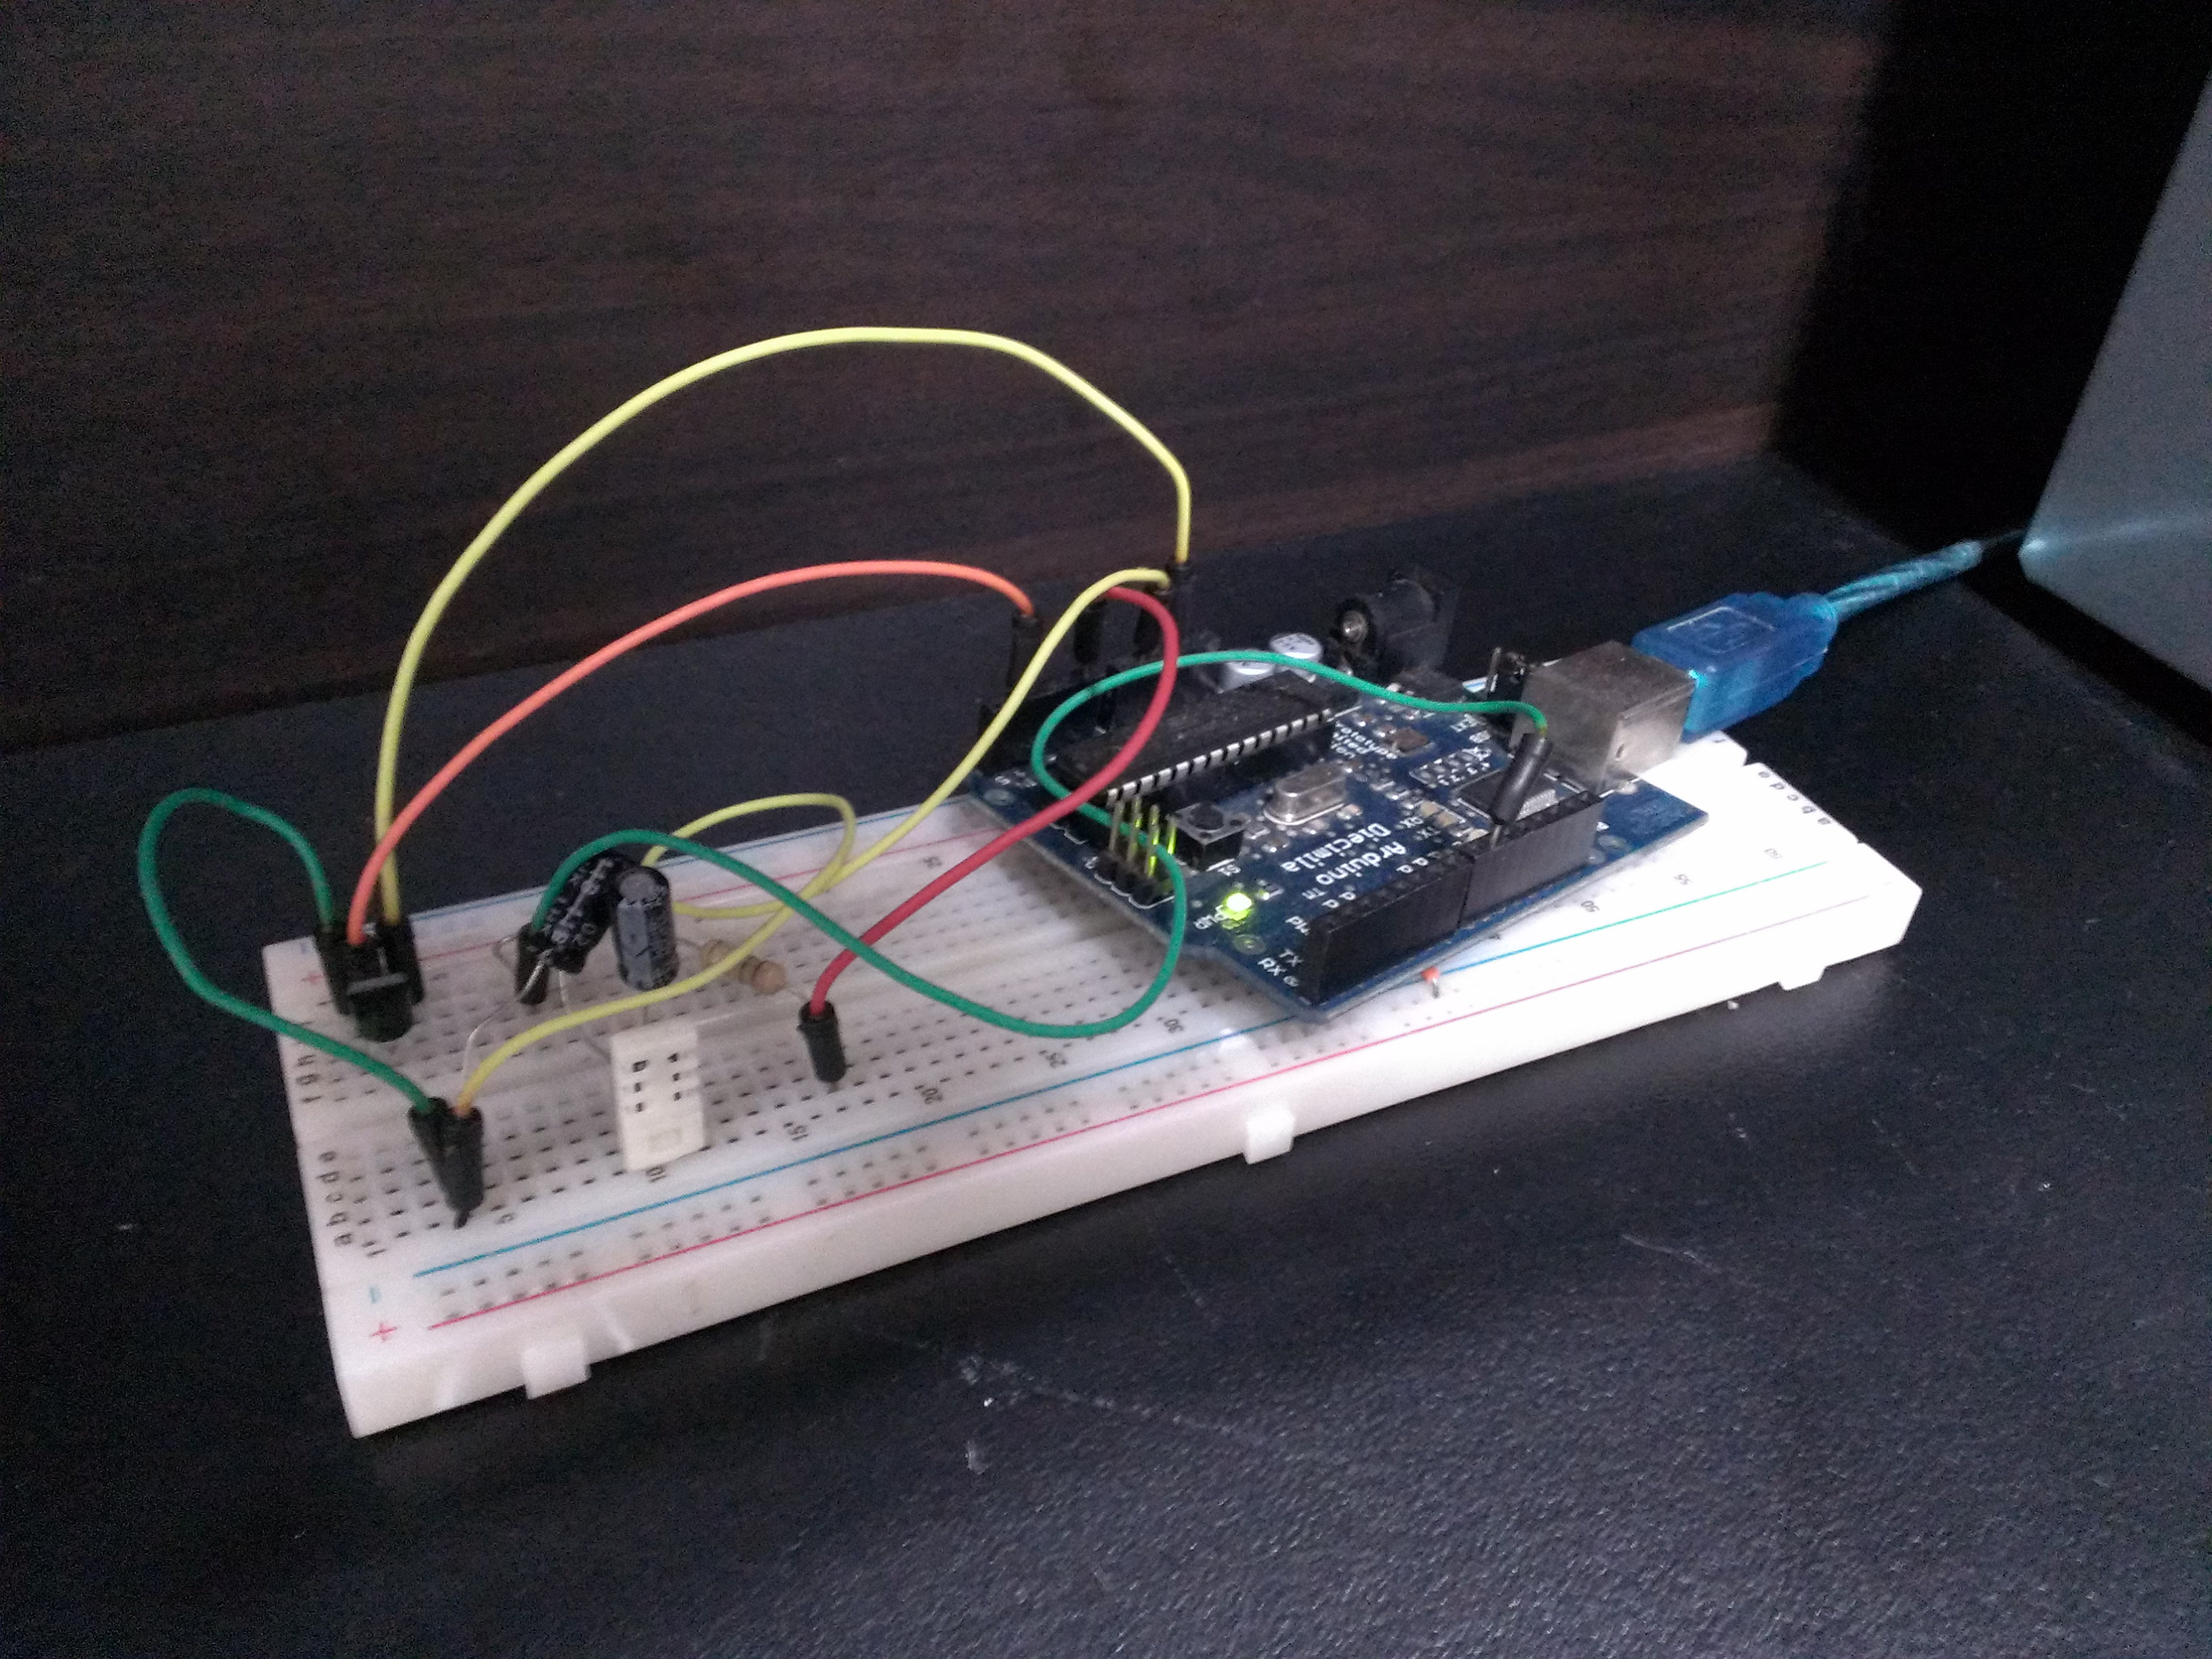
\includegraphics[width=140mm]{setup.jpg}
\caption{The entire setup on the breadboard}
\label{fig:setup}
\end{figure}

\section{Store and display}

On a server computer a Node.js application server gathers the data, displays it on a web interface, and forwards to a database. The source code of that server is on the net\footnote{Server source code: \url{https://github.com/UltracoldAtomsLab/weatherstation/tree/master/server}}, and can be installed as it is usual with Node.js applications: install Node.js if not already (tested v0.8.16), download the source, run `npm install` in the source code directory to install the dependencies, create a new configuration file from `config.json.default` into `config.json` (need to add the appropriate MongoDB server information).

The handled data is in JSON format, with 3 fields: `date`, `humidity`, `temperature`.

The current results are available to see on \url{http://hostname:5000/} where `hostname` is the appropriate hostname for the computer running the program.

The database is running MongoDB \, like other monitoring systems for the bakeout, just different database. The recorded weather values are currently kept for 2 weeks set by the appropriate Time-To-Live (TTL) values \footnote{Expiring data: \url{http://docs.mongodb.org/manual/tutorial/expire-data/}}.

\section{Weather report}

The weather report emails are handled by a Python script, that is scheduled to run at regular intervals (once a day). The source code is on the net as well\footnote{Weather report: \url{https://github.com/UltracoldAtomsLab/weatherreport}}. Tested with Python 2.7.3.

The resulting report graphics looks like Figure \ref{fig:weatherreport}, which includes humidity and temperature time series for the last 24h by default. The temperature measurement is smoothed by a Kalman-filter\footnote{Current implementation based on \url{http://www.scipy.org/Cookbook/KalmanFiltering}.} (in the `smooth.py` library also included), to reduce the measurement noise and find a more accurate running average. The Kalman filter has only one parameter, the process variance, that is just choosen empirically to give relatively smooth output for the given data, and its value is not critical.

\begin{figure}[ht!]
\centering
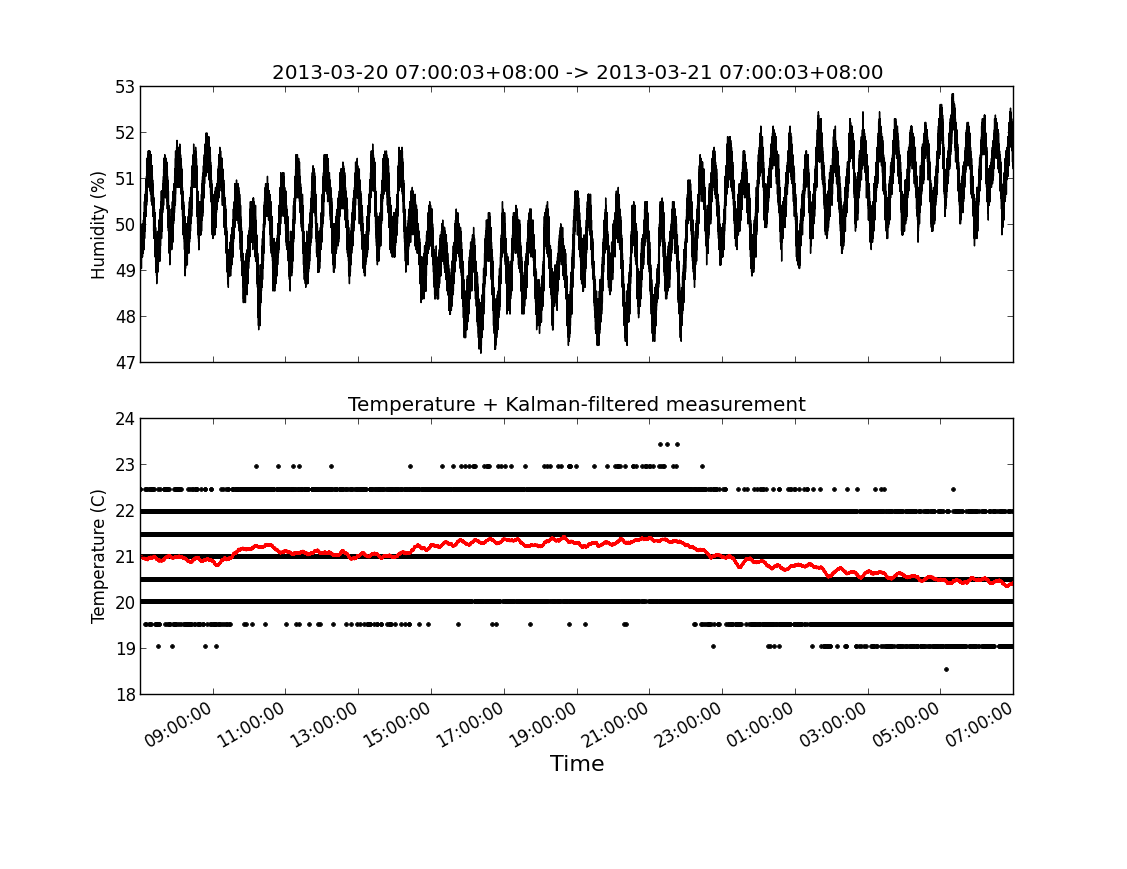
\includegraphics[width=140mm]{20130321-0700.png}
\caption{Example of weather report, for 2013-03-21 07:00:00}
\label{fig:weatherreport}
\end{figure}

When installing, a `weather.conf` file has to be created based on `weather.conf.example`, to set the correct configurations for the script. The configuration options (the database server, time zone, email settings) are named appropriately, and also commented.

The running of the script at regular intervals is done by cron (one common scheduler on Linux), have to set the following values in the cron config (with `crontab -e`):
\begin{lstlisting}[language=Bash,frame=single]
0 7 * * * /home/lab/prog/weatherreport/report.sh
\end{lstlisting}
which means that every day, at 7:00am run the following script. A quick analysis and report can be set by just running the script at any time, it will take the last 24h data. In such use case, might want to change the `weather.conf` temporarily to limit the email recepients (can comment out any line with placing `\#` as the first character, but make sure that when done, the original settings are restored).

The sending server's details are also set in `weather.conf`, see comments, right now it is set up to work with GMail + SMTP, using the lab account `yjlinlab@gmail.com`. Make sure that the password is never checked into the source control system.

\section{Troubleshooting}

If not sure whether the weatherstation is collecting data, could connect to the MongoDB Primary server (with the command `mongo hostname:port` with the appropriate hostname and port number) issue two simple commands: `use datasetname` where datasetname is the name of the dataset used in the settings (at the moment it is `weather`, thus the command is `use weather`. The next step is querying the latest reading in the database: \\`db.readings.find().sort({date: -1}).limit(1)`\\
This should return a result, and the date of that result should be recent (less than 5 seconds old). Take into account that the date is stored in UTC format (signified by the Z at the end the ISO 8601\footnote{ISO 8601: \url{http://en.wikipedia.org/wiki/ISO_8601}} formatted date), thus being 8 hours behind Taiwan!

For example the result in the Mongo shell, where rs0:PRIMARY$>$ is the MongoShell command prompt, signifying that one is connected to the Primary server of the replica set called `rs0`, and things after the $>$ sign are the ones that are typed, new lines are the results:
\begin{lstlisting}[language=sh,frame=single]
rs0:PRIMARY> use weather
switched to db weather
rs0:PRIMARY> db.readings.find().sort({date: -1}).limit(1)
{ "_id" : ObjectId("51626b1f6124d94bdcd5247d"),
"date" : ISODate("2013-04-08T07:00:47.936Z"),
"temperature" : 26.37, "humidity" : 48.41 }
\end{lstlisting}


\end{document}
